\subsection{Modeling the R-Transform}
\label{sxn:r_transforms}

To apply \SETOL, the model satisfy the \TRACELOG condition--which occurs during the case of  \IdealLearning.
For most cases of NN models, the ESD are HT; and this, in practice, one usually would select $R(x)$ that reflects this.
But to be more general, we formally extend the theory to allow the practioners to
both model the ESD as just a collection of discrete spikes, and to even correct for
\CorrelationTraps and/or \VeryHeavyTailed (VHT) ESDs.
Most importantly,  we derive expressions for both the~\WW~\ALPHA and~\ALPHAHAT metrics, valid
for the case \IdealLearning where $\alpha=2$, and formally extended for other cases.

The goal of this section is to obtain formal expressions for the \LayerQuality, $\Q$ which is
given in terms of what we somewhat imprecisely refer to as a \GEN.
In many cases, however, the resulting approximate expressions for $\Q$ do take the
form well-known norms, including the Frobenius norm, the Spectral norm, and the Shatten norm.
The models for $R(z)$  we use are presented in Table~\ref{tab:known_r_transforms} ,and
the final expression for the \LayerQuality $\Q$ for each model are given in Table~~\ref{tab:htsr_layer_quality}.

\subsubsection{Elementary Random Matrix Theory}
\label{sxn:r_transforms:elementary_rmt}

We begin with some useful notions definitions from \RandomMatrixTheory.
%
Using the ESD $\rho(\lambda)$, defined as
\begin{equation}
\label{eqn:rgo}
\rho(\lambda):=\frac{1}{N}\sum_{i}\delta(\lambda-\lambda_{i})  ,
\end{equation}
%
we can express the \emph{\GreensFunction} (or \emph{\CauchyStieltjes} transform $C(z)$) by%
\footnote{Please notice our naming and sign convention in \EQN~\ref{eqn:Cz}.
We equate the \GreensFunction $G(z)$ with
the (positive)\CauchyStieltjes transform, $G(z)=C(z)$.   Other works may use the opposite sign convention, $G(z)=-C(z)$.}
\begin{equation}
\label{eqn:Cz}
G(z)=C(z):=\int \mathrm{d}\lambda \frac{\rho(\lambda)}{z-\lambda} .
\end{equation}
%
From $G(z)$, we can recover the ESD, $\rho(\lambda)$, using the inversion relation
\begin{equation}
\label{eqn:GzInverse}
\rho(\lambda)=\lim_{\epsilon\rightarrow 0+}\frac{1}{\pi}\mathrm{IM}(G(\lambda+i\epsilon))  ,
\end{equation}
where $\mathrm{IM}$ is the imaginary part of $G(z)$, and where the $\lim_{\epsilon\rightarrow 0+}$ means to take the limit approaching from the upper half of the complex plane.
%
The \RTransform, $R(z)$, can be defined using the Blue function $B(z)$ 
\begin{equation}
\label{eqn:Rz}
R(z):=B(z)-\frac{1}{z}  ,
\end{equation}
where the Blue function $B(z)$~\cite{Zee1996} is the functional inverse of the Greens Function $G(z)$,% 
\footnote{The Blue function was first introduced by Zee~\cite{Zee1996} to model, among other things, spectral broadening in quantum systems.
Briefly, given a deterministic Hamiltonian matrix $\mathbf{H}_{0}$, with eigenvalues $\lambda^{0}_{i}$,
one can model the spectral broadening of $\lambda^{0}_{i}$ by adding a random matrix $\mathbf{H}_{1}$ to $\mathbf{H}_{0}$:
$\mathbf{H}=\mathbf{H}_{0}+\mathbf{H}_{1}$.  
The resulting eigenvalues of $\mathbf{H}$ now contain some level of randomness, $\sigma$, i.e., $\lambda=\lambda^{0}+\sigma$.  
To model the ESD of $\mathbf{H}$, one then specifies the invididual \RTransforms for $\mathbf{H}_{0}$ and $\mathbf{H}_{1}$; the full ESD of $\mathbf{H}$
can then be reconstructed by adding the two \RTransforms together $R(z)=R_{0}(z)+R_{1}(z)$.
Zee also notes that $R(z)$  is the same as the self-energy $\Sigma(z)$ from quantum many body theory~\cite{Zee1996}.}
satisfying 
\begin{equation}
\label{eqn:GzRelation}
B[G(z)]=z  .
\end{equation}
By specifying the $R(z)$ transform, we specify the complete ESD, $\rho(\lambda)$.
Here, we are actually only interested in the tail of $\rho(\lambda)$.
%and we can accept errors in $R(z)$ that describe the bulk region inaccurately or improperly. 
That is, we can given $R(z)=R(z)_{tail}+R(z)_{bulk}$, we only need $R(z)\approx R(z)_{tail}$.
\michaeladdressed{Good point to make here, but we need to make clear that our bulk/tails are not their bulk/tails.}
\charles{@michael: who is 'they' ?  }

\charles{Describe $R(z)$ is a power series, and how we take $\int dz R(z)$ and why we restirct the integral, contours, etc}



\subsubsection{Known \RTransforms and Analytic (Formal) Models}
\label{sxn:r_transforms:known_r_transforms}

There only a few known analytic results for the explicit \RTransform $R(z)$.
The ones we need are in Table~\ref{tab:known_r_transforms}.
Below, we review some of them, explaining what ESD they correspond to,
and what the resulting \GEN~$G(\lambda)$ would be if applied
as a model $R(x)$ here.
1;95;0c% Rtable.tex
\begin{table}[h!]
  \centering
  \renewcommand{\arraystretch}{1.25} % Increase line spacing in table
\begin{tabular}{|c|c|c|}
  \hline
  Model & \textbf{HTSR Universality Class} & \textbf{$R(z)$}\\  \hline
  \hline
  Discrete & Bulk$+$Spikes, MHT, HT & $\tfrac{1}{\MECS}\sum_{i=1}^{\MECS}\lambda_{i}$   \\ \hline
  \hline
  Wishart Models & &\\ \hline
  Multiplicative-Wishart & HT/VHT& $\dfrac{\epsilon\phi z^2}{2 - \epsilon\phi^2 z^2}$ \\  \hline
  Inverse Marchenko-Pastur & HT/VHT &  $\dfrac{\kappa-\sqrt{\kappa(\kappa-2z)}}{z}$   \\  \hline
  \hline
  L\'evy Wigner (LW) &   & \\  \hline
  Free Cauchy (FC) ($\alpha_{l}=1$) & HT $\alpha=2$ & $a+i\gamma$ \\ \hline
  General L\'evy  ($\alpha_{l}\ne 1$) & VHT $\alpha<2$   & $a+bz^{\alpha-2}$ \\  \hline
\end{tabular}
  \caption{Known \RTransforms for random matrix ensembles relevant to modeling heavy-tailed spectral densities (eigenvalues or singular values squared).
    The \emph{Multiplicative-Wishart} model has two real, non-zero parameters, $\epsilon$ and $\phi$; for more details,
    see \cite{PW16_NIPS}.
  For the \emph{\InverseMP}, as given by Bun~\cite{BunThesis}, $\kappa=\frac{1}{2}(Q-1)$ where, $q=\frac{1}{Q}=\frac{M}{N}\le 1$.
  The \emph{L\'evy-Wigner} (LW) model describes Wigner-like square random matrices
  (as opposed to Wishart-like or Correlation Matrices), where the elements are drawn from a L\'evy-Stable distribution.
  The resulting LW ESD is Heavy-Tailed Power Law, and characterized by the L\'evy exponent $\alpha_{l}$.
  The LW $R(z)$ is parameterized by a (real) shift parameter $a$,
  a complex phase factor $b$ (that depends on 3 real parameters   $\alpha_{l}, \beta$, and $\gamma$),
  and, of course, $\alpha_{l}$.
  The Free Cauchy (FC) model is a special case of the IW model, corresponding to the L\'evy $\alpha_{l}=1$, and the \HTSR $\alpha=2$. 
  We will extend the LW models to the rectangular case for our modeling purposes here by making
  the association   $\alpha = \alpha_{l}+1$ for $\alpha\le 2$.
  %$\alpha=\tfrac{1}{2}(\alpha_{l}+1)+1$ for $\alpha\le 2$.
   (Also, wwe take thew variance $\sigma=1$ for all models.)
   Generally speaking, the L\'evy $R(z)$ are more complicated; 
   for more details, see~\cite{BJNx01_TR,BJNx06_TR,BJ09_TR}.
}
\label{tab:known_r_transforms}
\end{table}



\charles{Discuss the Table briefly, and then each model in its own subsubsection.
We can create plots to show how these models can treat heavy tails, and explain the parameter fitting
}
\michael{We have five rows in the table but three subsubsxns below. How many do we have? Maybe make each a par rather than a subsubsxn.}
\charles{@michael: this is low priority, can revisit later}

\subsubsection{Discrete Model: Bulk$+$Spikes, MHT, HT}

Here, we consider modeling the  tail ESD, $\rho_{tail}(\lambda)$, as a collection
of discrete spikes $\lambda_{spike}$, 
where $\lambda_{spike}\ge \LambdaECSmin$.
This could be for modeling an ESD in the Bulk$+$Spikes \HTSR Universality class,
or it could be applied to an MHT or HT ESD as a discrete distributoon with
no inherent structure; its a modeling choice.
Here, \RTransform for the \ECS is sum of Dirac delta functions.
This lets us compute the \LayerQuality $\Q$ in closed form in terms of the Teacher weight matrix
$\TMAT=\WMAT$ as a Tail norm, the Frobenius norm of the tail eigenvectors.

Let the tail of the ESD have $\MECS = M^{tail}$ eigenvalues that define the \ECS, i.e.,  
\begin{equation}
\label{eqn:spikes_model_0}
\rho_{tail}(\lambda)=\sum_{i=1}^{\MECS}\delta(\lambda-\LambdaECS_{i}) .
\end{equation}
where the $\LambdaECS_{i}$ are normalized by $\tfrac{1}{M}$.

The \GreensFunction $G(z)$ is then
\begin{equation}
\label{eqn:spikes_model_1}
G(z) = \int d\lambda \dfrac{ \rho_{tail}(\lambda) }{z - \lambda} =
\sum_{i=1}^{\MECS} \int d\lambda \dfrac{\delta(\lambda-\LambdaECS_{i}) }{z - \lambda} =
\sum_{i=1}^{\MECS} \dfrac{1}{z-\LambdaECS_{i}}  ,
\end{equation}
and the Blue function for each individual term $i$ is $\frac{1}{z-\LambdaECS_{i}}$, i.e., $B(z)=\LambdaECS_{i}+\frac{1}{z}$. 
Now, using the additive property of the \RTransform, we can express the total $R(z)$ as the sum of the \RTransforms for the individual terms $i$, giving
\begin{equation}
\label{eqn:spikes_model_2}
R(z) =\sum_{i=1}^{\MECS}\left(\left(\LambdaECS_{i}+ \dfrac{1}{z}\right) - \dfrac{1}{z}\right)=\sum_{i=1}^{\MECS}\LambdaECS_{i}  .
\end{equation}
This gives the \GEN~$\GN$ as
\begin{align}
\label{eqn:spikes_model_3} 
\GN 
&= \int_{\LambdaECSmin}^{\lambda}\sum_{i=1}^{\MECS}\LambdaECS_{i} d\lambda \\ \nonumber
&= \sum_{i=1}^{\MECS}\LambdaECS_{i} \int_{\LambdaECSmin}^{\lambda} 1 d\lambda \\ \nonumber
&= \left(\sum_{i=1}^{\MECS}\LambdaECS_{i}\right)\left(\lambda-\LambdaECSmin\right)
\end{align}
Seeing that $\LambdaECSmin$ is usually quite small, we make the approximation
\begin{align}
\GN  \approx \left(\sum_{i=1}^{\MECS}\LambdaECS_{i}\right)\left(\lambda\right)  ,
\end{align}
which gives the \QualitySquared approximately as
\begin{align}
  \label{eqn:spikes_model_4}
  \QT = \sum_{i=1}^{\MECS}\GNECSI 
 \approx\left(\sum_{i=1}^{\MECS}\LambdaECS_{i}\right)^{2}  .
\end{align}
We now see that we can define $\Q:=\sqrt{\QT}=\sum_{i=1}^{\MECS}\LambdaECS_{i}$ is what we call a Tail Norm,
the Frobenius norm of the tail eigenvalues.

\subsubsection{Free Cauchy Model (\texorpdfstring{$\alpha = 2$}{alpha = 2})}
\label{sxn:r_transforms:free_cauchy}

For the \emph{Free Cauchy} (FC) model the \RTransform is a constant
\begin{equation}
\label{eqn:free_cauchy_R}
R(z)[\mathrm{FC}] = a + i\gamma ,
\end{equation}
where the shift parameter $a>0$ translates the FC spectrum (i.e. so it overlaps with the the Power Law tail of the ESD),
and the scale parameter $\gamma>0$ sets the tail width.
We do not attempt to fit $a$ and $\gamma$ to a real-world ESD here but rather simply use this model formally,

Because $R(z)$ is independent of $z$, the integral is straightforward:
\begin{equation}
\label{eqn:free_cauchy_G}
\GN[\mathrm{FC}] = \int_{\LambdaECSmin}^{\lambda} R(z)[\mathrm{FC}]dz = (a + i\gamma)(\lambda - \LambdaECSmin).
\end{equation}

%As above with the IW model, taking the modulus removes the phase factor in the $\GNECSI$, giving,
As explained in Appendix~\ref{sxn:tanaka}, when $R(z)$ is complex,  we keep the \emph{Real} part $\GNECSI$, giving,
\begin{equation}
\label{eqn:free_cauchy_G_abs}
\Re[\GN[\mathrm{FC}]] = a(\lambda - \LambdaECSmin).
\end{equation}

To obtain a formal expression for $\ALPHA$, we make two approximations.
First, we take the lower cut-off to be near zero $(\LambdaECSmin \approx 0)$.
\begin{equation}
\label{eqn:free_cauchy_G_max}
\bigl|\GN[\mathrm{FC}]\bigr|_{\LambdaECSmin \approx 0} \approx a\lambda
\end{equation}
Second, we assume the \LayerQualitySquared is dominated by the largest term in the sum:
\begin{equation}
\label{eqn:free_cauchy_G_max2}
\QT_{\mathrm{FC}} = \sum_{i=1}^{\MECS}\bigl|\GN[\mathrm{FC}]\bigr|_{\LambdaECSmin \approx 0}
= a\sum_{i}^{\MECS} \LambdaECS_{i} \approx a\lambda_{max}
\end{equation}

For the Heavy-Tailed ESDs, we genrally find that as $\lambda_{\max}$ increses, the \HTSR $\alpha$ decreases.
Juat for illustrative purposes,
If we take $\log_{10}\lambda_{\max}\sim\frac{1}{\alpha}$ (assuming $\log_{10}\lambda_{\max}>1$), and take the square root of both sides,
we obtain the desired result for the log \Quality, namely, that it scales inversely with $\alpha$
\begin{equation}
\label{eqn:free_cauchy_Q}
\log_{10}\Q_{\mathrm{FC}} \sim \frac{1}{\alpha}
\end{equation}

If we extend this formally beyond the Ideal  case to $\alpha\ge 2$, we now can exlain why the \HTSR $\alpha$
makes a good \LayerQuality metric in deep networks,
as smaller $\alpha$ suggests higher quality layers and therefore a higher overall model quality and/or accuracy. 


\subsubsection{Inverse Marchenko-Pastur Model of \IdealLearning}
For a more realistic model of a layer ESD, 
here, we consider the \InverseMP (IMP) model.\cite{BunThesis}
The IMP model treats the ESD of $\mathbf{X}^{-1}$ when the ESD of $\mathbf{X}$ itself is MP.
As a parametiric model, it can be quite effective at treating VHT and HT (or \FatTailed) ESDs,
$\alpha\le 4$, but works best whenb $\alpha=2.0$.
To do this, one simply considers  $\kappa$, and the variance, $\sigma^2$ (not shown), as an adjustable paremeters.
%
It is an excellent model for the ESD when $\alpha=2.0$ (and $Q=2$).
Using this model, we can derive an expression for the \HTSR \ALPHAHAT \LayerQuality metric,
$\ALPHAHATEQN :=\ALPHAHATLONG)$ as a leading order term in the final expression for $\log_{10}\QT$.

\begin{figure}[h]
    \centering
    \subfigure[IMP Distribution, $\kappa=0.5$]{ 
      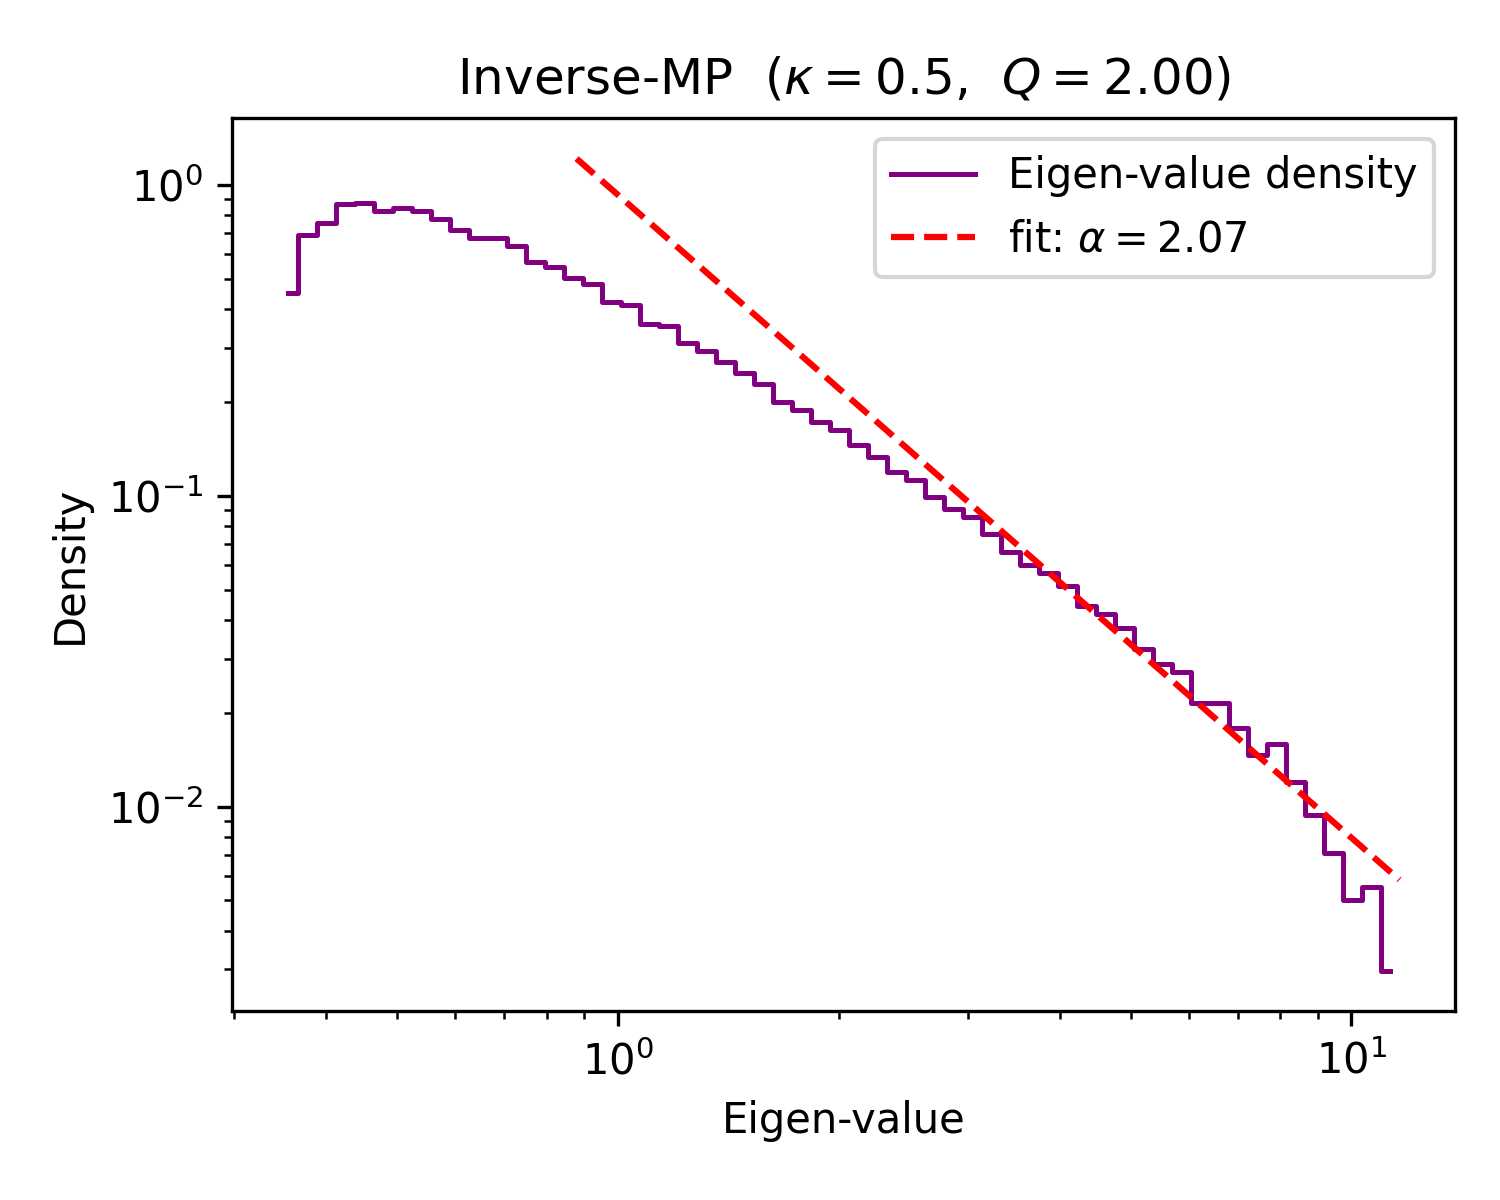
\includegraphics[width=7.5cm]{./img/IMPplotKappa0.5.png}
      \label{fig:IMPplotESD}                               
    }                               
      \subfigure[IMP $\kappa$ vs. \HTSR $\alpha$]{ 
      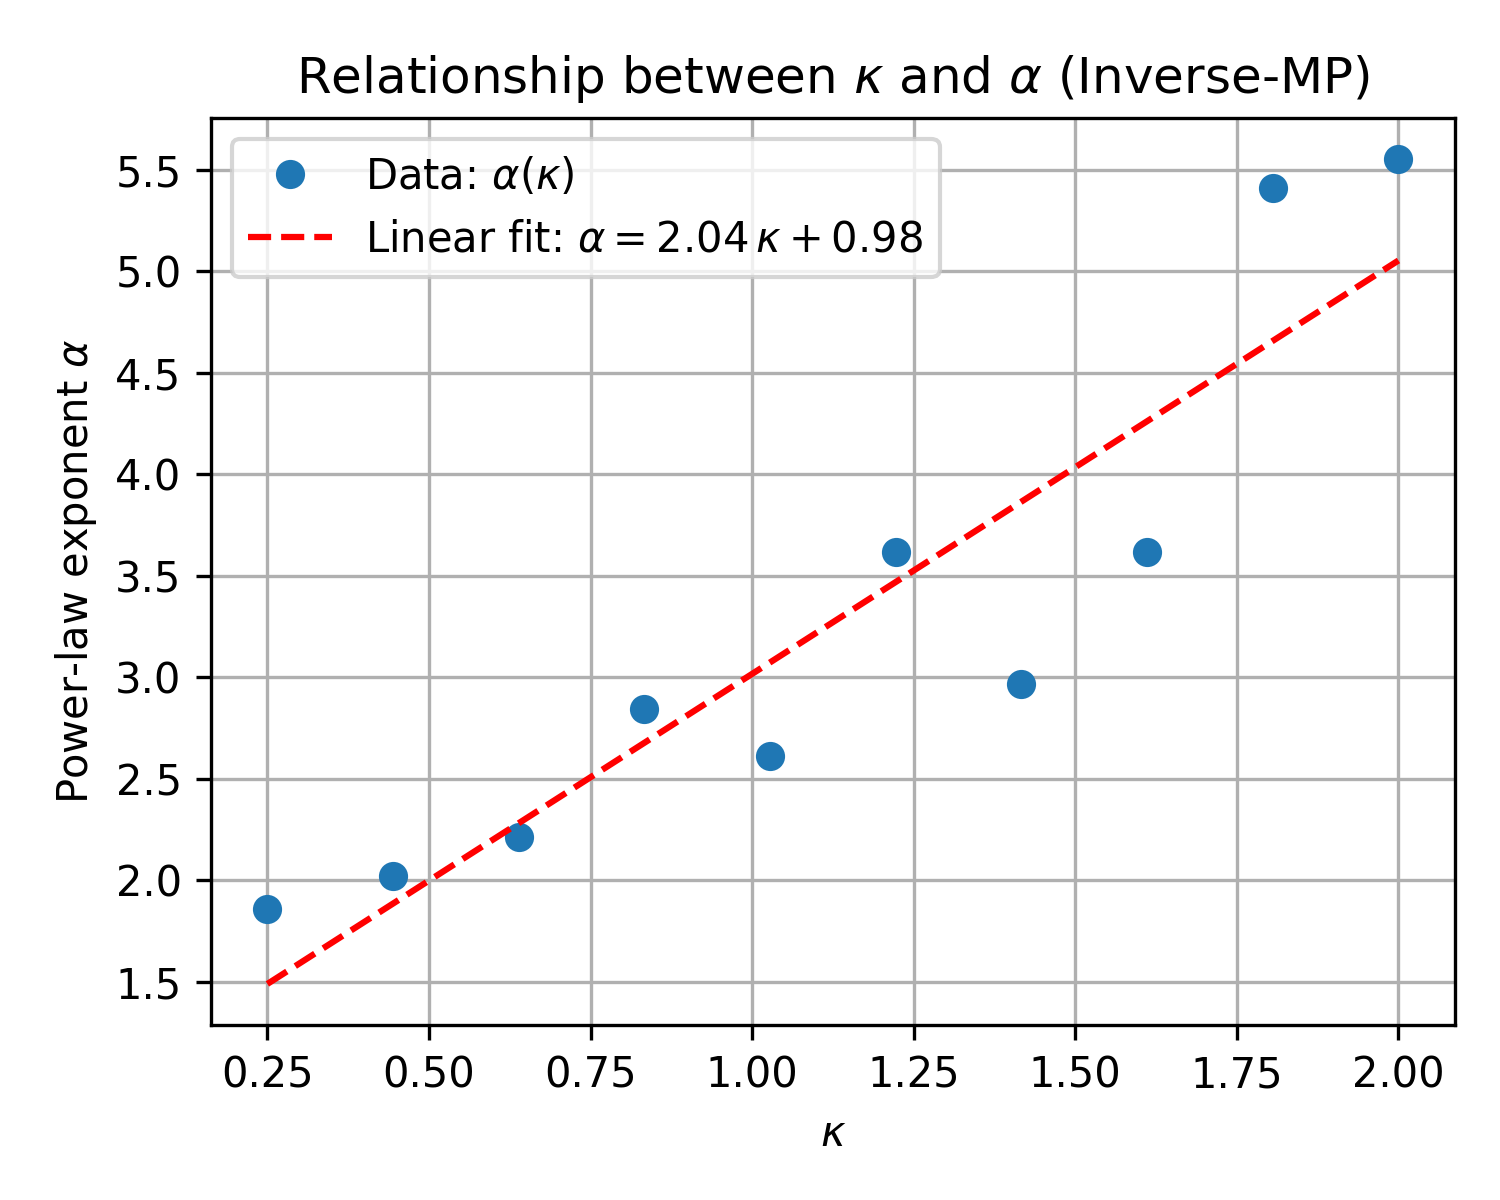
\includegraphics[width=7.5cm]{./img/kappa_vs_alpha_with_fit.png}
      \label{fig:IMPPlotKappaVsAlpha}                                
      }
      \caption{
        (\ref{fig:IMPplotESD}) plots a typical \InverseMP (IMP) ESD  $\kappa=0.5$,  along with Power Law (PL) fits, with PL exponent$\alpha=1.86$.
        (\ref{fig:IMPPlotKappaVsAlpha}) depicts the linear relationship betweem $\kappa$ and $\alpha$.
      }
  \label{fig:IMPplots}                                                                                                      
\end{figure}   

In Figure~\ref{fig:IMPplots}, we generate a random IMP model ESD with $\kappa=0.5$, $Q=2.0$, fit the ESD
to a PL, and find $\alpha=1.08$; this is a reasonably accurate model of an PL ESD for $\alpha\approx 2$.
For larger $\kappa$, the fits are not as good, but the model is stil useful to suggest a heurstic model for the
\LayerQuaiityy in terms of the \HTSR $\alpha$.
In Figure~\ref{fig:IMPPlotKappaVsAlpha}, we show that there is a simple relationship betweem $\kappa$ and $\alpha$,
which allows us to formally state $\alpha=2\;\kappa$.

\begin{figure}[t]
    \centering
    \subfigure[IMP $R(z)$, real $z$.]{
        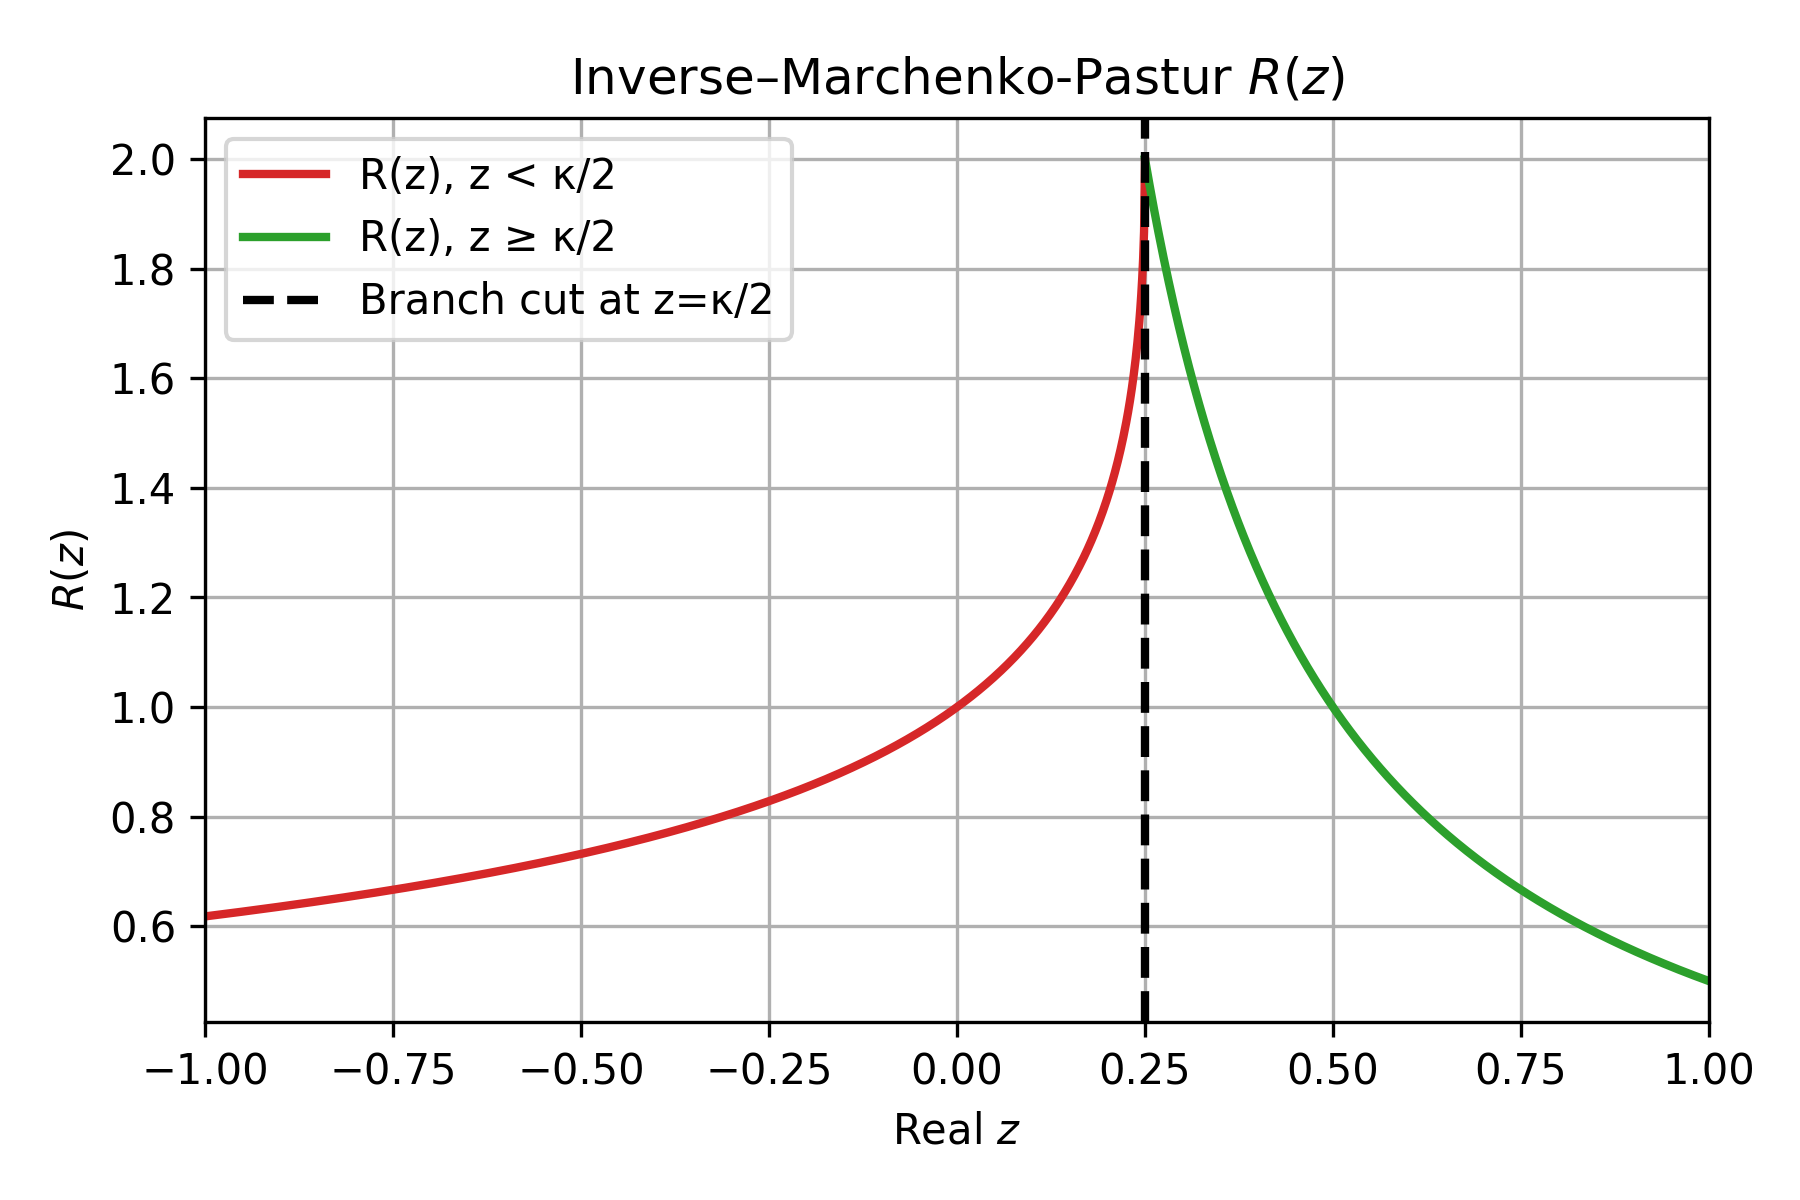
\includegraphics[width=7.5cm]{img/IW_R_transform_sides.png}
        \label{fig:IMP_R}
    }
    \subfigure[Branch cut at $z=\kappa/2$]{
        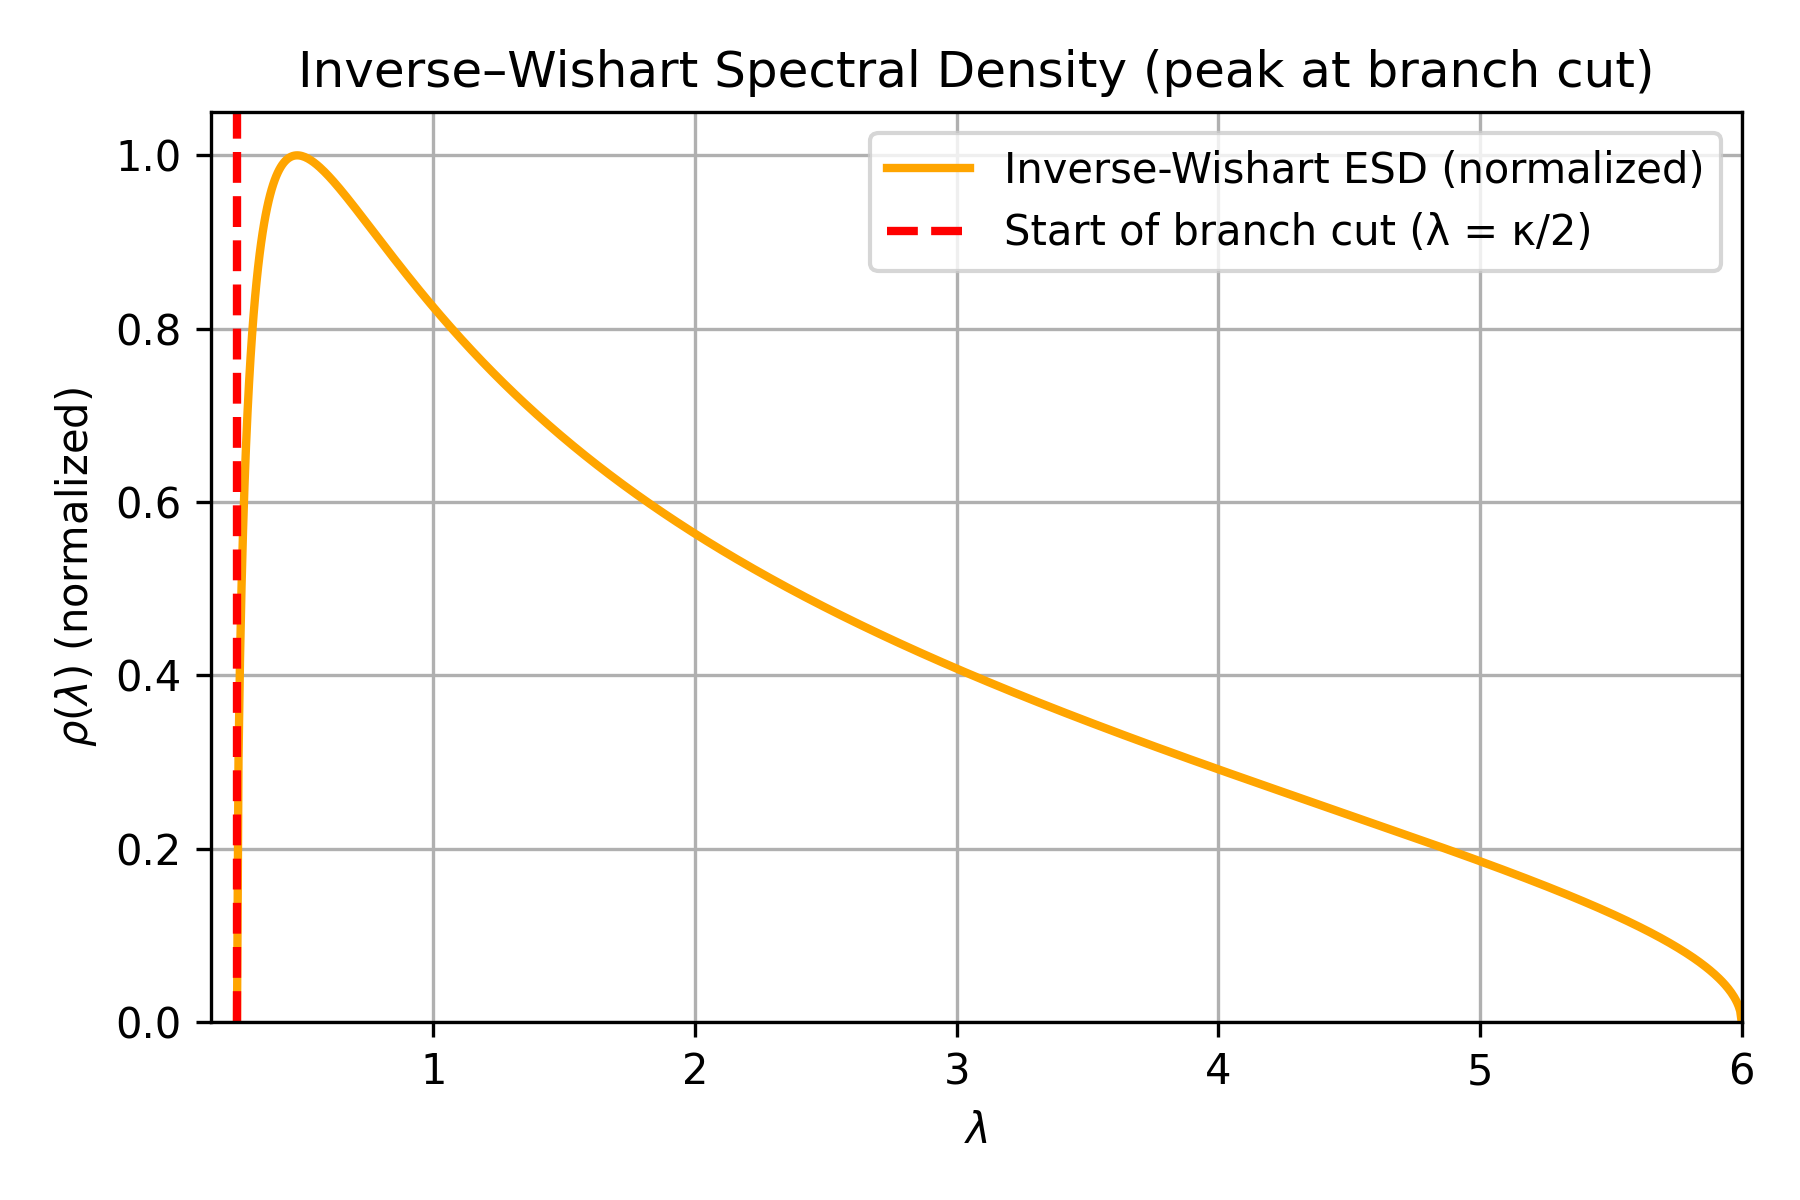
\includegraphics[width=7.5cm]{img/Branch_Cut_Density_normalized.png}
        \label{fig:IMP_branch_cut}
    }
    \caption{(a) The function $R(z)$ of the \InverseMP (IMP) model, with a singularity at $z = \kappa/2$. (b) The branch cut in the Empirical Spectral Density (ESD) at $\kappa = 0.5$.}
    \label{fig:R_branch_cut_combined}
\end{figure}

Lets consider $R(z)$ for the \InverseMP model, denoted $R(z)[IMP]$.
To integrate this function, we require that it be analytic.
At first glance, it may seem that that $R(z)[IMP]$ is not analytic because it
has a pole at $z=0$ and because the square-root term $\sqrt{\kappa(\kappa-2z)}$  creates branch
cut at and $z=\kappa/2$ (and $z=\infty$).
Figure~\ref{fig:R_branch_cut_combined} presents this in two ways:
Figure~\ref{fig:IMP_R} shows the R-transform $R(z)[IZ]$ for real $z$, highlighting its singular behavior and the location of the branch cut at $z = \kappa/2$; and
Figure~\ref{fig:IMP_branch_cut} shows the corresponding branch cut in the ESD of the Inverse MP model (for $\kappa = 0.5$).
We select the branch cut starting at $z=\kappa/2$ and ending at $z=\infty$,
which allows us to at least formally defined the integral along the physically meaningful part of the ESD:
\begin{equation}
\label{eqn:IMP_model_1} 
\GN[\mathrm{IMP}] := \int_{\LambdaECSmin}^{\lambda} \Re[R(z)][\mathrm{IMP}] dz  ,
\end{equation}
noting that we expect $\LambdaECSmin\ge\kappa/2$ and we take the \emph{Real} part of $R(z)$, $\Re[R(z)]$.

It turns out, however, that due to the branch cut in $R(z)[\mathrm{IMP}]$,
the function $\GN[\mathrm{IMP}]$ is not analytic in the domain we need. 
To correct for this, we will instead model the \LayerQualitySquared using the \emph{Real Part} $\Re[\GN[\mathrm{IMP}]]$,
which yields (See Appendix~\ref{sxn:IMP}):
\begin{equation}
  \label{eqn:IMP_model_2}
G(\lambda)[IMP] = \int_{\LambdaECSmin}^\lambda \frac{\kappa}{z} , dz = \kappa \left[ \ln z \right]_{\LambdaECSmin}^\lambda = \kappa \left( \ln \lambda - \ln \LambdaECSmin\right).
\end{equation}
Notice this expression is very similar to the expression for the Free Cauchy model above (\EQN~\ref{eqn:free_cauchy_G_max2}), except
now it is terms of the logarithm of $\lambda$, and rescaled by $\kappa$.
By associating $\alpha=2\;\kappa$, we recover the \ALPHAHAT formular, albeit with a different normalization .

\subsubsection{The Multiplicative-Wishart (MW) model}
The Multiplicative-Wishart (MW) model  has two real, adjustable parameters $\epsilon,\phi$.
It treates $\mathbf{X}$ as resulting from product of random matrices, and is good for modeling an ESD with a Very Heavy Tail (VHT).
It has been used previously to model the heavy tail of the Hessian matrix in NNs\cite{Pennington2017}
This model would work better for fitting HT ESDs that decay slower than a PL or TPL.
We note that unlike the IMP, the MW model does not have a branch cut at the ECS, but it does
have $2$ poles, compicating the integration of the  \RTransform.
We will not consider this model further here and instead leave this for future work.


\subsubsection{Levy-Wigner Models and the \ALPHAHAT Metric}

eHere, we consider General Levy-Wigner (LW) model..
We show how to obtain the \WW~\ALPHAHAT metric by modeling VHT ESDs with an approximation to a Levy distribution, suitable
for cases where the \HTSR $\alpha\le 2$.  

The~\ALPHAHAT metric has been developed to adjust for \SCALE anomalies that arise from issues like \CorrelationTraps,
rank collapse, and overfitting, which can in many cases make \ALPHA smaller than expected, and even smaller than $2$.
We model these VHT ESDs  \emph{as if} they follows a Levy-Stable distribution, generated from a \LevyWigner random matrix.
The  \LevyWigner (LW) model treats  $\mathbf{X}$ as if it were a \Wigner matrix (and not actually a rectnalgyle correlation  matrix),
s we must decide how to map the \HTSR $\alpha$ to the L\'evy $\alpha_{l}$; for this, we select $\alpha_{l}=\alpha-1$.
(See in Table~\ref{tab:known_r_transforms}.)
The LW model is defined in terms of 3 paremeters:
$a$ is a shift parameter, and $b$ is a complex phase factor depending on 2 real factors, $\beta$ and $\gamma$.
Strictly the ESD for an LW model, $\rho_{LW}(\lambda)$, is defined by its characteristic function (i.e., the Fourier Transform of $\rho_{LW}(\lambda)$), but we  when the ESD is VHT, $\rho_{LW}(\lambda)\sim\lambda^{-\alpha_{l}-1}$, and  when $\alpha_{l}\approx 1$, the ESD resembles a PL HT ESD with the \HTSR $\alpha\approx 2$.

Let us model the \RTransform of our \VeryHeavyTailed (VHT) ESDs as
\begin{align}
\label{eqn:LW_model_0} 
R(z)[\mathrm{LW}] & = bz^{\alpha_{l}-1},\;\alpha_{l}\in(0,1) \\ \nonumber
  & = bz^{\alpha-2},\;\alpha\in(0,2),
\end{align}
where $b$ is an unspecified constant (possibly negative and/or complex).
This is not a particualry good model for VHT ESDs in practice; it is simply an approximate model
we choose to obtain a formal expresion.

Integrating $R(z)[\mathrm{LW}]$, and (as above) taking the approximation $\LambdaECSmin\approx 0$, we obtain 
\begin{equation}
\label{eqn:LW_model_1} 
\GN[\mathrm{LW}] \approx \tfrac{b}{\alpha-2} \lambda^{\alpha-2}  .
\end{equation}
%
For simplicity, if we now choose $b=\alpha_{l}=\alpha-2$, then  $\QT_{\mathrm{LW}}$ takes the form of a Shatten Norm
\begin{equation}
  \label{eqn:LW_model_2}
  \QT_{\mathrm{LW}} = \frac{1}{\MECS}\sum_{i}^{\MECS}\lambda^{\alpha-1}  .
\end{equation}
%
Taking the logarithm of $\QT_{\mathrm{HT}} $, we obtain 
\begin{equation}
\label{eqn:LW_model_3} 
\log \QT[\mathrm{LW}] \approx (\alpha-1)\log\lambda
\end{equation}

As with the Free Cauchy (FC), let us approxmate $\QT$ by the largest term in the sum over $\GNECSI$, and then let $\lambda=\lambda_{max}$, giving
\begin{equation} 
\label{eqn:LW_model_4} 
\ALPHAHATEQN = \log_{10} \QT_{\mathrm{LW}} \approx (\alpha-1)\log\lambda_{max}   .
\end{equation}
We present this as a formal example, noting that is slightly different from the result for the IMP model, Eqn.~\ref{eqn:IMP_alphahat}. 
We do not claim this is a valid empirical model, as we have not attempted to fit a real-world ESD to Levy-stable distribtion.  
\michael{Let's sync on the rationale here, since I'm not sure what is being said.}
We leave this to a future study, noting, however, there has been some work doing such fits~\cite{li2024exploring}.

Ideally, we would like to have an rigorous expression for $R(z)$ not just
in the case of \IdealLearning but also for the entire \FatTailed Universality class.
This is non-trivial to obtain and we will attempt this in a future work.
Fow now, we will take a different approach, and evaluate $R(z)$ explicitly using numerical techniques.

\paragraph{Scaling insight.}
For the VHT Universality class, we may expect $\lambda_{\max}$ to be fairly large such that
$\lambda_{max}>1$ and therefore $\log_{10}\lambda_{max}>0$
This implies that  $\log_{10}\QT$ decreases  as $\alpha$ (and thus $\alpha_l$) decreases, even though
$\log_{10}\lambda_{max}$ simultaneously \emph{increases} in the VHT class.
This opposing interplay explains why correlation traps produce small $\alpha$ yet yield deceptively moderate quality scores.

\paragraph{Historical remark.}
An earlier study on \ALPHAHAT,reported the opposite trend, with $\ALPHAHAT$ decreasing with increasing model quality.
This is because we employed an un–normalised covariance, suggesting that $\lambda_{max}<1$ and $\log_{10}\lambda_{max}<0$
(although we have not rigorously checked this).
The present $M$ normalisation clarifies that the VHT regime is meaningful \emph{only} when $\alpha<2$,
indicating the layer amd therefore the model is overfit (in some unspecified way).


\subsubsection{Summary of heurstic models.}
Using the results for different \RTransforms, we can construct several different, related heurstic models for the \LayerQuality
that resemble the very successful \WW \HTSR \ALPHA and \ALPHAHAT metrics.  These heurstic models allow us extend
the \SETOL results for \Ideal learning (i.e. $\alpha=2$) to a wider range of NN layers, covering the \HTSR
HT and VHT Universality classes and, correspondingly, NN layers that are both underfit $(\alpha>2)$
and overfit $(\alpha<2)$.

% Gtable.tex  —  final closed-form (or leading-order) Layer Quality \Q
\begin{table}[h!]
  \centering
  \renewcommand{\arraystretch}{2}
  \small
  \begin{tabular}{|c|p{2.5cm}|c|p{4.5cm}|}
    \hline
    \textbf{Model} & \textbf{Metric} & \textbf{$\log\Q$ (Approx.\ Log Quality)} & \textbf{Interpretation} \\ \hline\hline

    Delta Function (Spikes)
      & Tail Norm
      & $\displaystyle \log\l\sum_{i=1}^{\MECS}\LambdaECS_{i}$
      & The Frobenius-like Tail norm sums the $\LambdaECS_{i}$ in the \ECS. \\ \hline

    Free Cauchy (FC)
      & \ALPHA $\alpha$
      & $\displaystyle \log\lambda_{max}\sim\frac{1}{\alpha}$
      & The log \Quality scales as $\tfrac{1}{\alpha}$, showing why smaller $\alpha$ yields higher $\Q$. \\ \hline

    L\'evy Wigner (LW)
      & \ALPHAHAT $\hat{\alpha}$ 
      & $\displaystyle (\alpha-1)\,\log\lambda_{\max}
        \;+\;\mathrm{const.}$
      & Similar to \ALPHAHAT, heavier tails ($\alpha\in(1,2)$) depress \LayerQuality. \\ \hline

    Inverse Wishart\footnotemark
      & ECS Boundary
      & $\displaystyle 0.5\log\lambda_{\max}
        \;+\;\mathrm{const.}$
      & Branch cut defines the \ECS \\ \hline

  \end{tabular}
  \caption{Closed-form or leading-order expressions for the log \LayerQuality
           $\log\Q$ derived from the integrated $R$–transform for each core
           tail-model, simplified to show the relation to the ~\WW~\ALPHA and ~\ALPHAHAT metrics. }
  \label{tab:htsr_layer_quality}
\end{table}

\footnotetext{See Appendix~\ref{sxn:IW}, Eq.\,(A.7.25): $|G(\lambda)|\approx1.138\,\lambda^{0.539}$.}

Table~\ref{tab:htsr_layer_quality} consolidates the derived expressions for the log \LayerQuality, \(\log\Q\), across multiple \(R\)–transform models, each capturing distinct heavy-tail characteristics of the ESD within the \SETOL framework. The Discrete (Spikes) model yields a Frobenius-like tail norm by summing the effective eigenvalues in the \ECS, directly tying quality to tail magnitude (cf.\ \EQN~\ref{eqn:spikes_model_4}). The Free Cauchy (FC) model links \(\log\Q\) inversely to the \HTSR metric \ALPHA, demonstrating that smaller \(\alpha\) values enhance quality (cf.\ \EQN~\ref{eqn:free_cauchy_Q}). The L\'evy-Wigner (LW) model connects \(\log\Q\) to \ALPHAHAT through the term \((\alpha-1)\log\lambda_{\max}\), revealing how very heavy tails depress layer quality (cf.\ \EQN~\ref{eqn:LW_model_4}). The Inverse MP (IMP) model defines the \ECS boundary via a branch cut at \(\kappa/2\) and approximates \(\log\Q\) as \(0.5\log\lambda_{\max}\), providing a robust metric for \IdealLearning scenarios. Each model thus offers a unique lens on layer quality, enabling direct mapping between theoretical \(R\)–transform assumptions and empirical \WW metrics.

\paragraph{Practical Implications for Neural Network Analysis}
These models empower researchers to tailor layer-quality assessments to specific \HTSR universality classes, boosting the predictive power of \WW metrics like \ALPHA and \ALPHAHAT. The Discrete model excels when the ESD exhibits clear eigenvalue spikes, delivering a sharp quality signal for Bulk$+$Spikes layers. The FC model supports \IdealLearning by linking quality directly to \(1/\alpha\), which simplifies cross-layer comparisons. The LW model helps detect overfitting by adjusting for \CorrelationTraps via \ALPHAHAT in very heavy-tailed regimes. Finally, the IMP model offers a parametric fit for both HT and VHT tails, with \(\kappa\) tuning alignment to real-world ESDs (cf.\ Figure~\ref{fig:IMPplots}). By integrating these models, practitioners can compute precise layer-quality metrics that optimize both performance and interpretability.
